% !TEX root = ..\main.tex
\chapter{Introduction}

\section{Motivation and Background}
The field of embedded systems is growing rapidly based on the evolution in electronics and widespread use of sensors and actuators. From consumer electronics to automobiles, to satellites, embedded systems represent one of the largest segment of the software industry. Our society has come to depend on such systems for its day-to-day operation, and with this trend ongoing, we clearly see that most future computing systems will be embedded systems\cite{wolfmadsen-2000}. Internet of Things describes the concept of interconnecting the virtual world of computers with the real world of physical artifacts\cite{mattern2010internet}. This leads to a distributed network of devices communicating with other devices as well as humans. Gartner has estimated that in 2020, 25 billion connected "things" will be in use\cite{gartner}. 

Software plays an important role in the development of embedded systems. The software is specialized for one particular type of hardware and may therefore have hardware specific run-time constrains. To provide more functionality, multiple components are combined together within embedded systems. However, as the complexity of embedded system increases, the ability to maintain the required quality of such systems becomes more difficult. Combination of multiple components leads to higher costs of verifying additional software and many consequencly may fail to test the product properly and deliver a reliable product.  

Embedded systems expected lifetime goes beoynd one decade for many systems, which requires managing old systems in parallell to the design and implementation of new systems. 


In most cases, many companies are forced to think about their time-to-market strategy to keep up with the increased competition. This leads companies to decide what shortcuts in the development process they have to take. Such compromises leads to the creation of a financial overhead in the future maintenance activities, usually termed as technical debt\cite{p29-cunningham}. 

As technical debt accumulates, it becomes necessary to manage the overall debt while keeping the system flexible and extensible. Companies must often recall their products. If they could catch software defects earlier in the system design process, they would have saved a lot of money. It is important to find out how to make decisisions so future maintenance and evolution has as low cost as possible. 


Technical debt is a rising problem. It is estimated that the cost of dealing with technical debt threatens to grow to \$ 1 trillion globally by 2015\cite{gartner2010}. That is the double of the amount of technical debt in 2010. IT management teams must measure the level of technical debt in their organization and develop a strategy to deal with it.

\begin{table}[H]
	\centering
	\begin{tabular}{ | l | l | l | l | l |}
	\hline
	\textbf{Category} & \textbf{2013} & \textbf{2014} & \textbf{2015} & \textbf{2020} \\ \hline
	Automotive & 96.0 & 189.6 & 372.3 & 3,511.1 \\ \hline
	Consumer & 1,842.1 & 2,244.5 & 2,874.9 & 13,172.5 \\ \hline
	Generic Business & 395.2 & 479.4 & 623.9 & 5,158.6 \\ \hline
	Vertical Business & 698.7 & 836.5 & 1,009.4 & 3,164.4 \\ \hline
	\textbf{Grand Total} & \textbf{3,032.0} & \textbf{3,750.0} & \textbf{4,880.6} & \textbf{25,006.6} \\
	\hline
	\end{tabular}
	\caption{Table from Gartner\cite{gartner}} \label{tab:table1}
\end{table}


\section{Research Questions}
The main objective of this project is to increase the knowledge on the significant sources of technical debt, and find out how technical debt in embedded systems are managed. The reason for this is that embedded systems usually has long lifetime, and it is important to find out how such systems are managed because the architecture and design decisions are usually made long time ago and the decision makers might not be available anymore. 

\textbf{The research questions will be:} 
\begin{itemize}
	\item \textbf{RQ-1}: What practices and tools for managing technical debt? How are they used?
	\item \textbf{RQ-2}: What are the most significant sources of technical debt?
	\item \textbf{RQ-3}: When should a technical debt be paid?
	\item \textbf{RQ-4}: Who is responsible for deciding whether to incur, or pay off technical debt?
\end{itemize}

\section{Research Method}
The most relevant research methologies in software engineering is summarized in Figure \ref{fig:researchProcess}. Throughout this thesis, the research process illustrated in the model will be used as a basis for the elaboration of how to conduct the research in my master thesis. 

\begin{figure}[H]
	\centering
	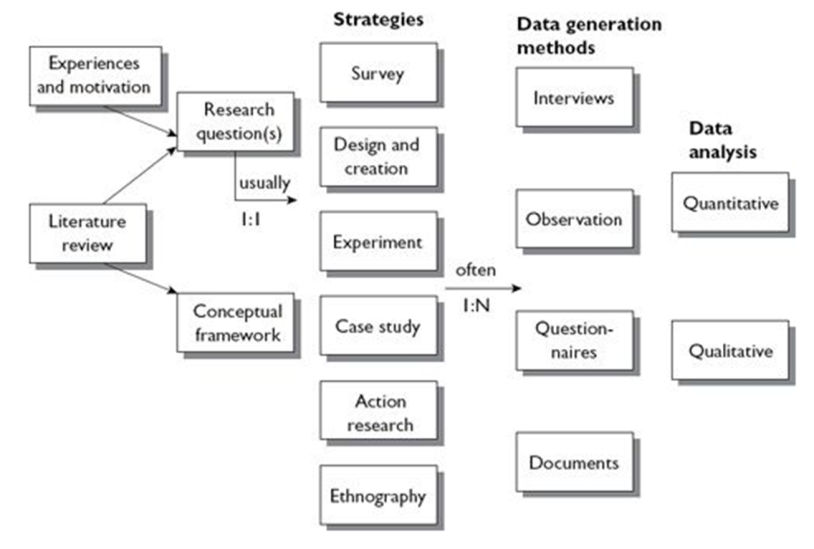
\includegraphics[width=0.8\textwidth]{images/researchStrategies.png}
	\caption{Model of research process\cite{Oates:2006:RIS:1202299}}
	\label{fig:researchProcess}
\end{figure}

To define the research questions, it is necessary to get an overview of the research field by conducting a review of published research within the selected area of study, or use experiences and motivations. This provides a conceptual framework for this research. A research strategy is needed to answer the research questions. There are six different research strategies: survey, design and creation, experiment, case study, action research, and ethnography. A data collection method is needed to produce empirical data or evidence. There are four methods: interviews, observations, questionnaire, and documents. These data can either be quantitative or qualitative. 

A litterature review was conducted to start with, providing a conceptual framework for this research. This led to the definition of the research questions to be answered in this research. To answer the research questions, survey is chosen as research strategy along with interviews for data collection.


\section{Project Structure}
The report is structured as follows:
\begin{itemize}
	\item \textbf{Chapter 1} introduces the problem and motivation behind this project, the research questions, and the different parts of this project.
	\item \textbf{Chapter 2} provides a state-of-art within the field of technical debt, embedded systems, and software engineering.
	\item \textbf{Chapter 3} presents the research method, and the procedures behind the method.
	\item \textbf{Chapter 4} provides an overview of the results and analyses from the research method.
	\item \textbf{Chapter 5} presents a discussion of the whole project.
	\item \textbf{Chapter 6} concludes the report and provides some points to future work. 
\end{itemize}

